\chapter{Конструкторский раздел}
\label{cha:design}

В данном разделе будет проведена конкретизация поставленных задач, составлены и проанализированы алгоритмы.

\section{Модель}
IDEF0 модель задачи вычисления произведения двух матриц представлена на рисунке 2.1.
\begin{figure}
    \centering
    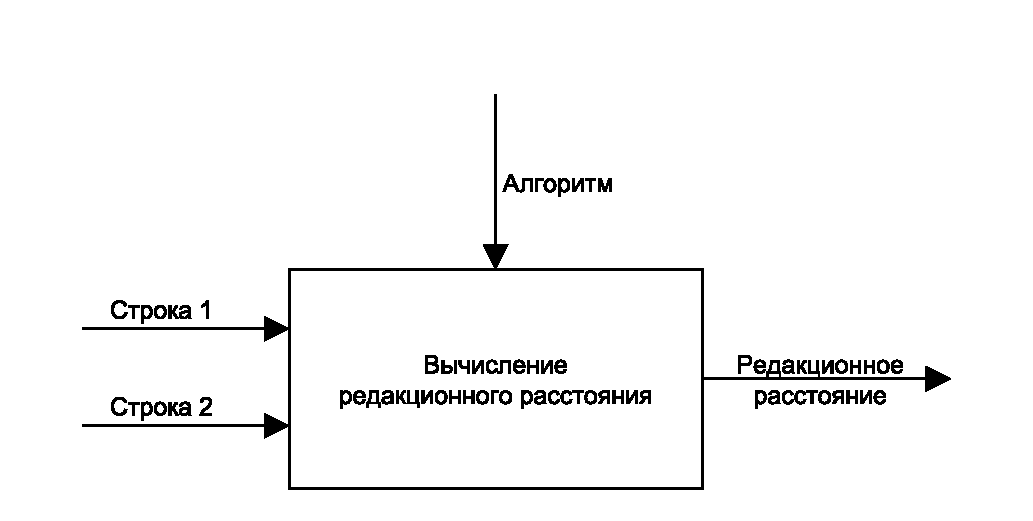
\includegraphics[scale=.7]{pdf/mainIdef0.pdf}
    \caption{IDEF0 модель}
\end{figure}

\section{Разработка алгоритмов}
Для непосредственной реализации вышеописанных алгоритмов важно иметь их некоторые упрощённые визуальные представления, так как чтение таких представлений упрощает написание кода. Подходящим для этого вариантом визуализации являются схемы алгоритмов.

\subsection{Классический алгоритм умножения матриц}
Схема классического алгоритма умножения матриц приведена на рисунке 2.2.
\begin{figure}[H]
    \centering
    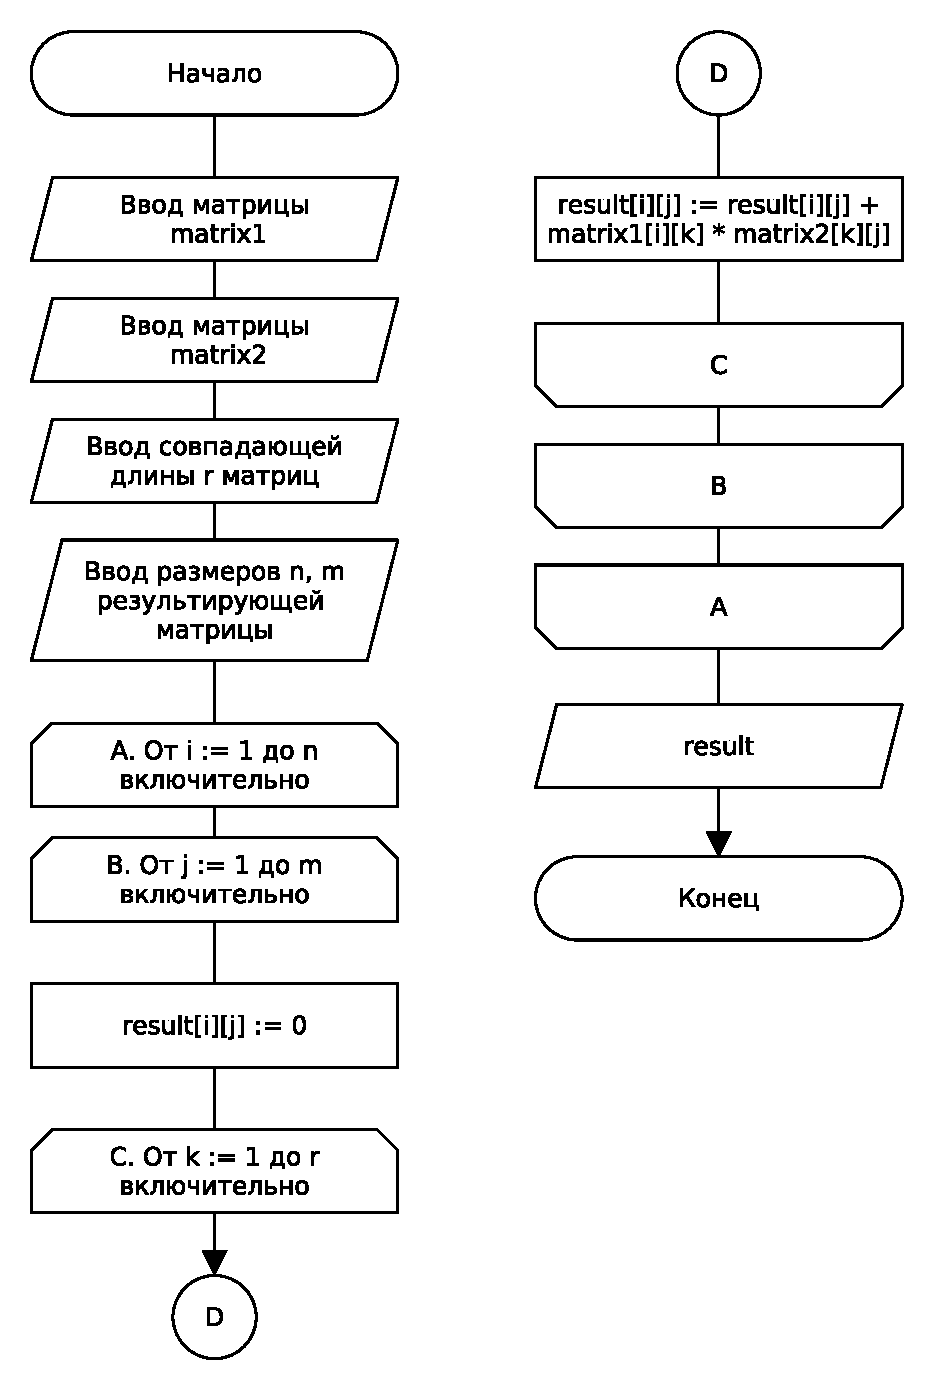
\includegraphics[scale=0.75]{pdf/classicmul.pdf}
    \caption{Классический алгоритм}
\end{figure}

\subsection{Алгоритм Винограда}
Схема алгоритма Винограда приведена на рисунках 2.3 и 2.4.
\begin{figure}[H]
    \centering
    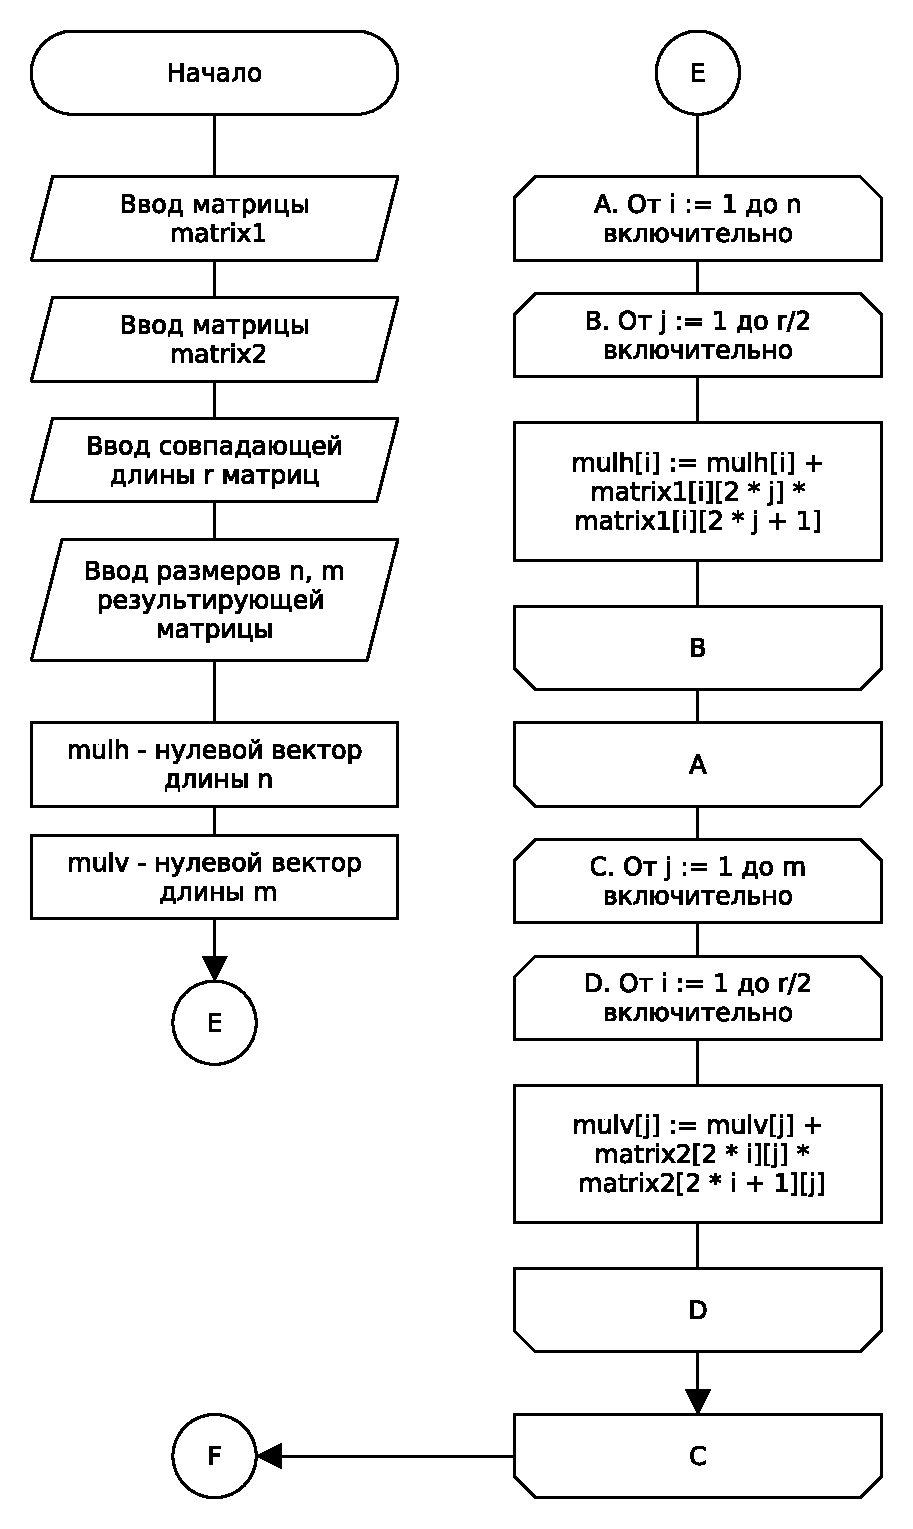
\includegraphics[scale=0.75]{pdf/winograd-part1.pdf}
    \caption{Алгоритм Винограда, часть 1}
\end{figure}

\begin{figure}[H]
    \centering
    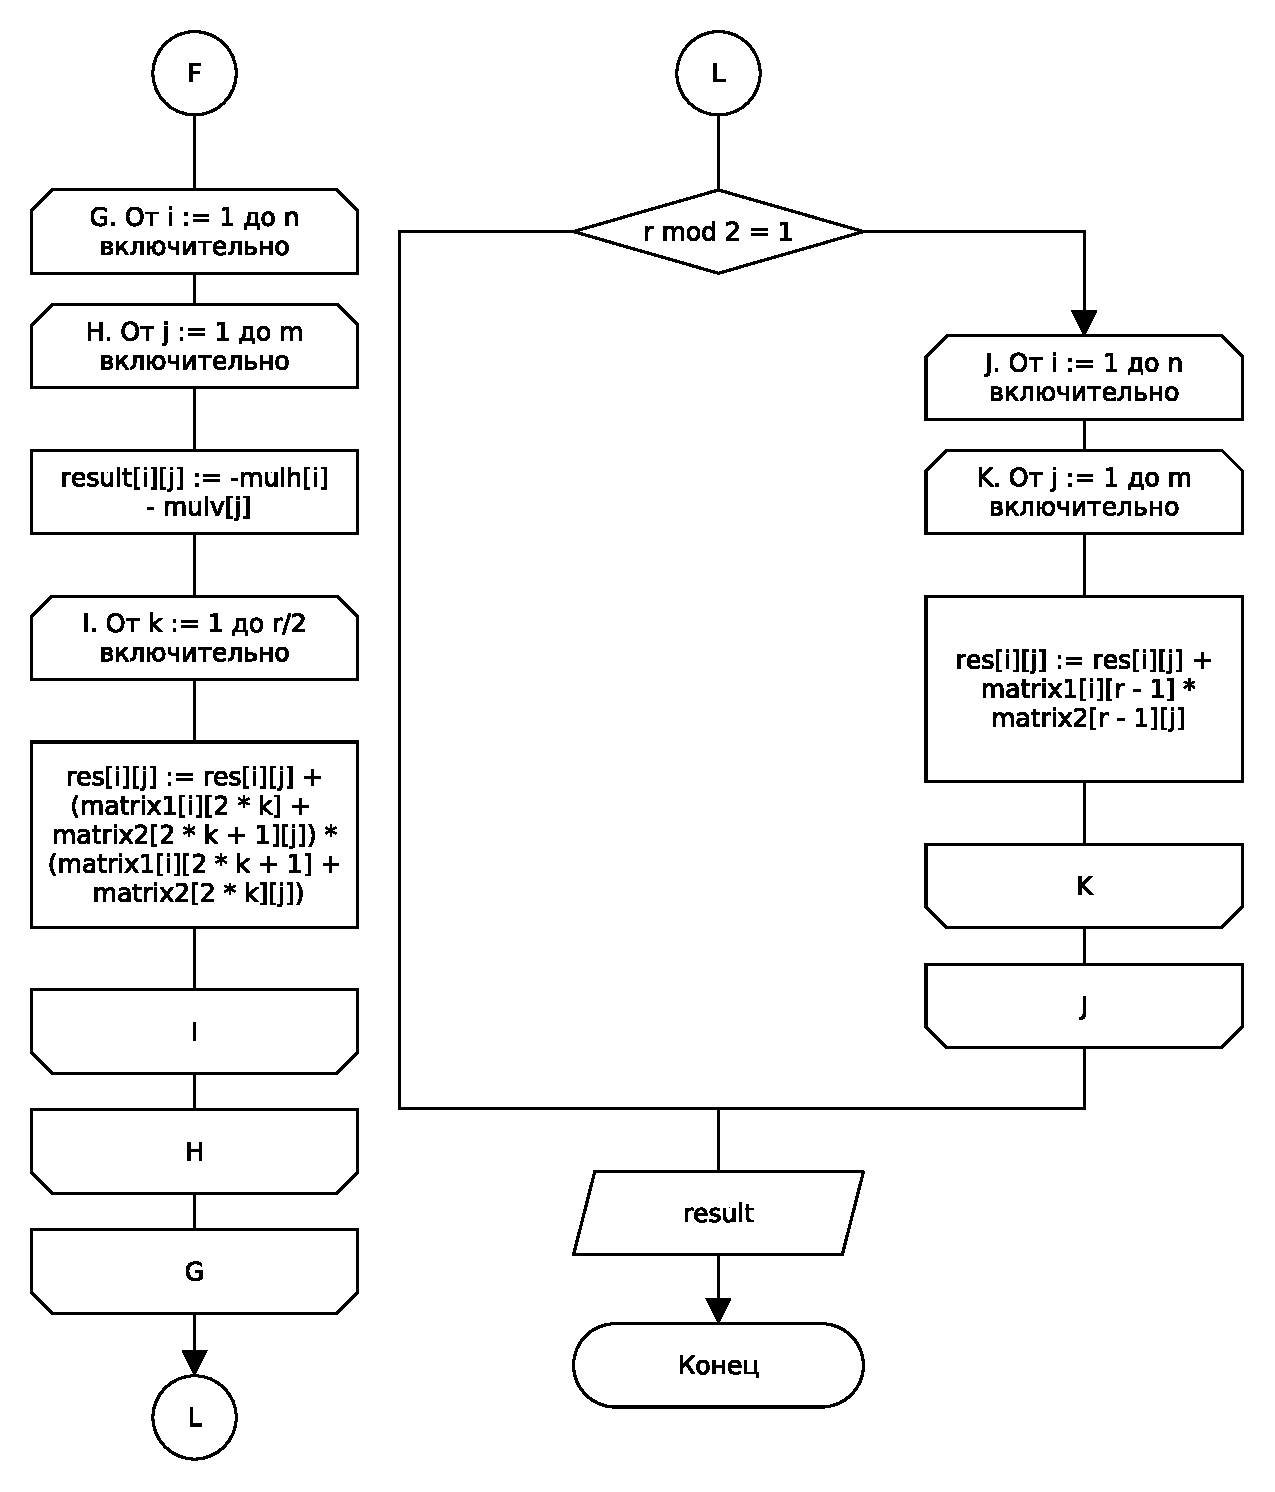
\includegraphics[scale=0.75]{pdf/winograd-part2.pdf}
    \caption{Алгоритм Винограда, часть 2}
\end{figure}

\section{Трудоёмкость алгоритмов}
Для того, чтобы произвести оценку трудоёмкости рассматриваемых алгоритмов, определим стоимость базовых операций:
\begin{itemize}
    \item операции стоимостью 0:
        \begin{itemize}
            \item условный переход;
        \end{itemize}
    \item операции стоимостью 1:
        \begin{itemize}
            \item операции сравнения;
            \item арифметическая унарная операция -;
            \item арифметические бинарные операции: +, -;
            \item операции инкремента и декремента;
            \item битовые операции;
            \item операции работы с памятью: разыменование, взятие адреса;
            \item операции присваивания: простая и сложные, совмещенные с операциями из этого списка;
        \end{itemize}
    \item операции стоимостью 2:
        \begin{itemize}
            \item арифметические бинарные операции: *, /, \%;
            \item операции работы с памятью: индексация;
            \item составные операции присваивания, совмещенные с другими операциями этого списка.
        \end{itemize}
\end{itemize}

Тогда стоимость выполнения си-подобного параметрического цикла for определяется стоимостью полей инициализации, условия и модификации его заголовка, а так же стоимостью тела этого цикла и количеством его  срабатываний.

\subsection{Классический алгоритм}
Оценим трудоёмкость классического алгоритма умножения двух матриц. Обозначения идентичны обозначениям на рисунке 2.2.

Данный алгоритм начинается с параметрического цикла от $i := 1$ до $n$. Значит, этот цикл сработает $n$ раз, а цена его заголовка составляет $1 + 1 + 1 = 1 + 2$, где цена инициализации составляет 1, а остальная цена заголовка равна 2. Подобных циклов всего 3 и каждый следующий вложен в предыдущий.

Внутри второго присутствует обращение к элементу матрицы и присваивание этому элементу значение 0. Стоимость этого выражения составляет $2 + 2 + 1 = 5$.

Внутри третьего цикла присутствует выражение, состоящее из 4 обращений к элементу матрицы, одного умножения, одного сложения и одного присваивания. Следовательно, его стоимость равна $4\cdot{}(2 + 2) + 2 + 1 + 1 = 20$.

Имеем итоговую стоимость всего алгоритма:
\begin{equation}
    \begin{gathered}
    1 + n \cdot{} (3 + m \cdot{} (3 + 5 + r \cdot{} (2 + 20))) =\\
    22nmr + 8nm + 3n + 1
    \end{gathered}
\end{equation}

\subsection{Алгоритм Винограда}
Теперь проведём оценку трудоёмкости алгоритма Винограда. Обозначения идентичны обозначениям на рисунка 2.3 и 2.4.

Как видно на рисунке 2.3, в начале схемы данного алгоритма присутствуют два однотипных двойных цикла. Для упрощения вычислений, рассмотрим  первый. В предыдущем пункте уже было объяснено, что стоимость заголовка такого цикла составляет 3, а выполнится он $n$ раз (инициализация выполняется всего один раз, поэтому 1 + 2n). Стоимость заголовка вложенного цикла выше на 2 - там присутствует операция целочисленного деления, а выполнится он $\frac{r}{2}$ раз. Внутри второго цикла находится только одно выражение, состоящее из из двух обращений к элементу матрицы, двух обращений к элементу вектора, трёх произведений, двух сложений и одного присваивания. Цена этого выражения равна $2\cdot{}(2 + 2) + 2\cdot{}2 + 3\cdot{}2 + 2\cdot{}1 + 1 = 21$. Стоимость всего цикла составляет:
\begin{equation}
    \begin{gathered}
        1 + n\cdot{}(3 + \frac{r}{2}\cdot{}(4 + 21)) = 12.5\cdot{}nr + 3n + 1
    \end{gathered}
\end{equation}
А стоимость следующего:
\begin{equation}
    \begin{split}
        1 + m\cdot{}(3 + \frac{r}{2}\cdot{}(4 + 21)) = 12.5\cdot{}mr + 3m + 1
    \end{split}
\end{equation}

Далее следует тройной цикл, с точки зрения структуры аналогичный описанному в предыдущем пункте, но с важными отличиями:
\begin{itemize}
    \item стоимость самого вложенного цикла выше на 2, так как в его условии присутствует дополнительная операция деления;
    \item самый вложенный цикл выполнится не за $r$ раз, а за $\frac{r}{2}$ раз;
    \item стоимость выражения, с которого начинается тело второго цикла, равна 11;
    \item стоимость выражения, из которого состоит тело третьего цикла, равна 37.
\end{itemize}
Стоимость всего цикла равна:
\begin{equation}
    \begin{gathered}
        1 + n\cdot{}(3 + m\cdot(3 + 11 + \frac{r}{2}\cdot{}(4 + 37))) = 20.5nmr + 14nm + 3n + 1
    \end{gathered}
\end{equation}

Схема данного алгоритма завершается ветвлением, результатом которого может быть всего два исхода: выполнение двойного цикла или пропуск этого цикла. Цена проверки условия этого ветвления составляет $2 + 1 = 3$. Стоимость заголовков и количество срабатываний следующих циклов ранее было вычислено: 3, $n$ раз и 2, $m$ раз соответственно. Выражение, находящееся во вложенном цикле, состоит из 4 обращений к элементу матрицы, одного умножения, двух вычитаний, одного сложения и одного присваивания. Значит, его стоимость равна $4\cdot{}(2 + 2) + 2 + 2\cdot{}1 + 1 + 1 = 22$. Тогда стоимость всего цикла равна:
\begin{equation}
    1 + n\cdot{}(3 + m\cdot{}(2 + 22)) = 24nm + 3n + 1
\end{equation}

Таким образом, можно подсчитать итоговую стоимость всего алгоритма:
\begin{equation}
    20.5nmr + 14nm + 12.5nr + 12.5mr + 6n + 3m + 6 + Z
\end{equation}
где
\begin{equation}
Z = \left\{ \begin{array}{ll}
 24nm + 3n + 1, & \textrm{если r нечётно}\\
 0, & \textrm{иначе}\\
\end{array} \right.
\end{equation}

\subsection{Модификация алгоритма Винограда}
Очевидно, что алгоритм Винограда при перемножении больших матриц будет работать быстрее классического алгоритма умножения. Но даже этот результат можно улучшить, произведя ряд модификаций:
\begin{itemize}
    \item замена комбинации операции присваивания и операции сложения на соответствующую составную операцию присваивания. Например, выражение вида $a = a + ...$ будет заменено на $a += ...$;
    \item замена операции целочисленного деления на 2 операцией битового логического сдвига вправо на 1. Аналогично с операцией целочисленного умножения на 2 и операцией битового логического сдвига влево на 1;
    \item замена в проверке на чётность операции получения остатка от деления на 2 на операцию побитового умножения на 1;
    \item перенос из условия цикла лишних вычислений во внешнюю область видимости;
    \item буферизация значений, записываемых в память посредством использования операции разыменования, при условии, что это происходит в цикле.
\end{itemize}

С учётом произведенных изменений, имеем схему улучшенного алгоритма Винограда на рисунках 2.5 и 2.6.
\begin{figure}[H]
    \centering
    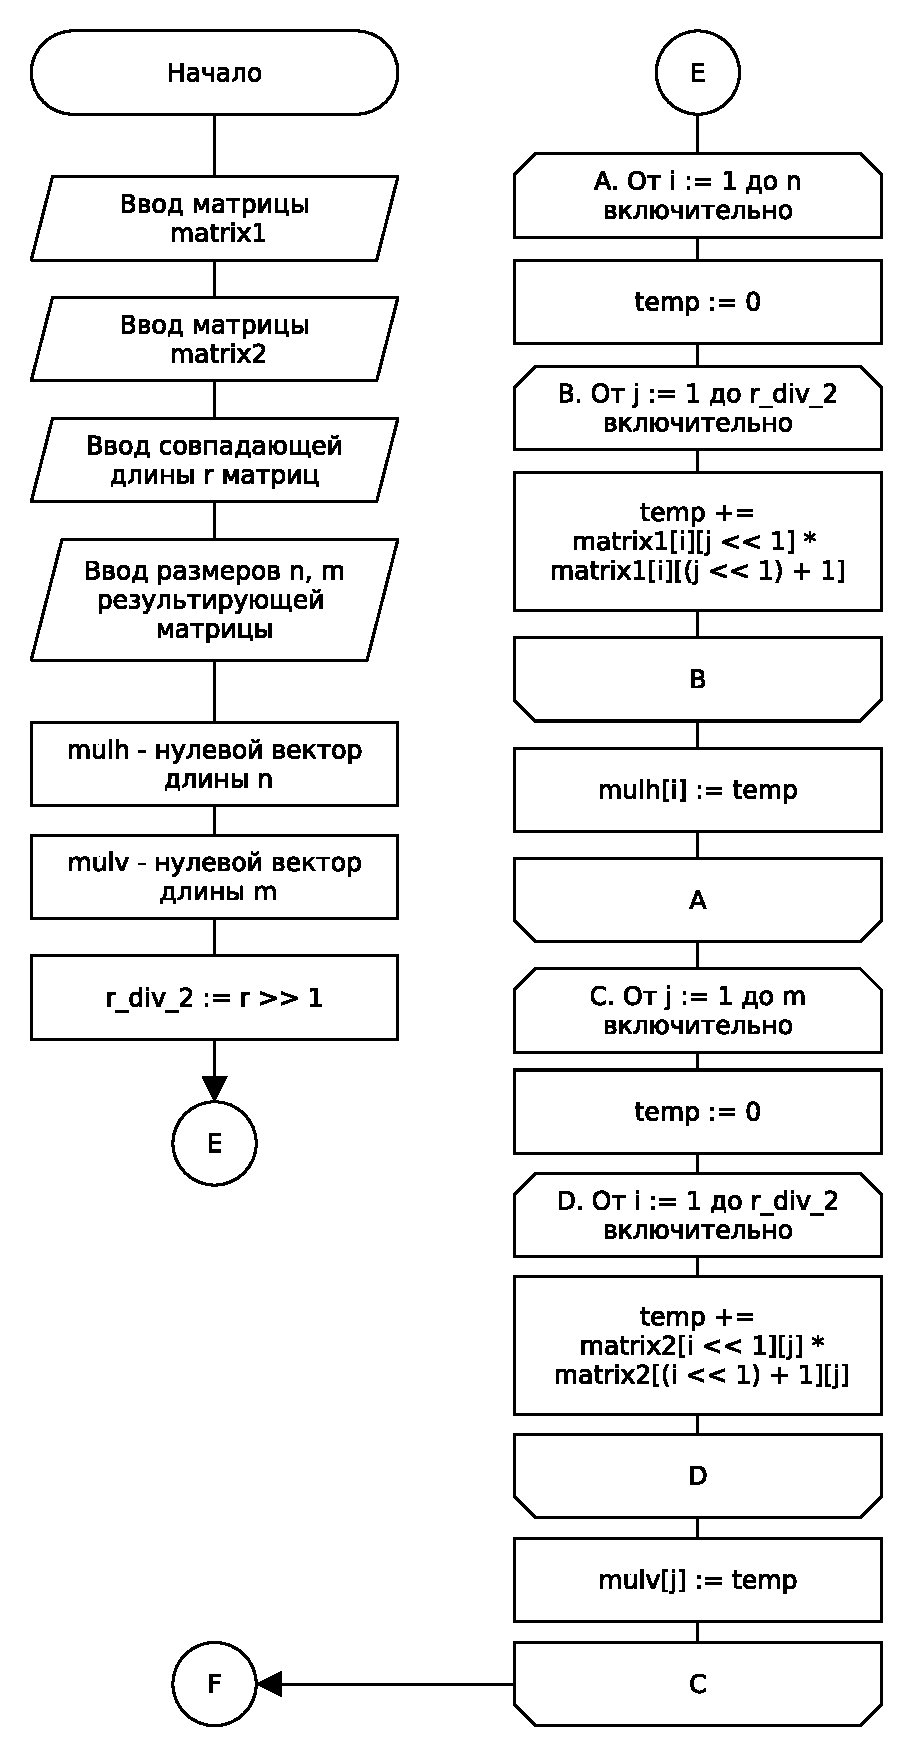
\includegraphics[scale=0.75]{pdf/owinograd-part1.pdf}
    \caption{Модифицированный алгоритм Винограда, часть 1}
\end{figure}

\begin{figure}[H]
    \centering
    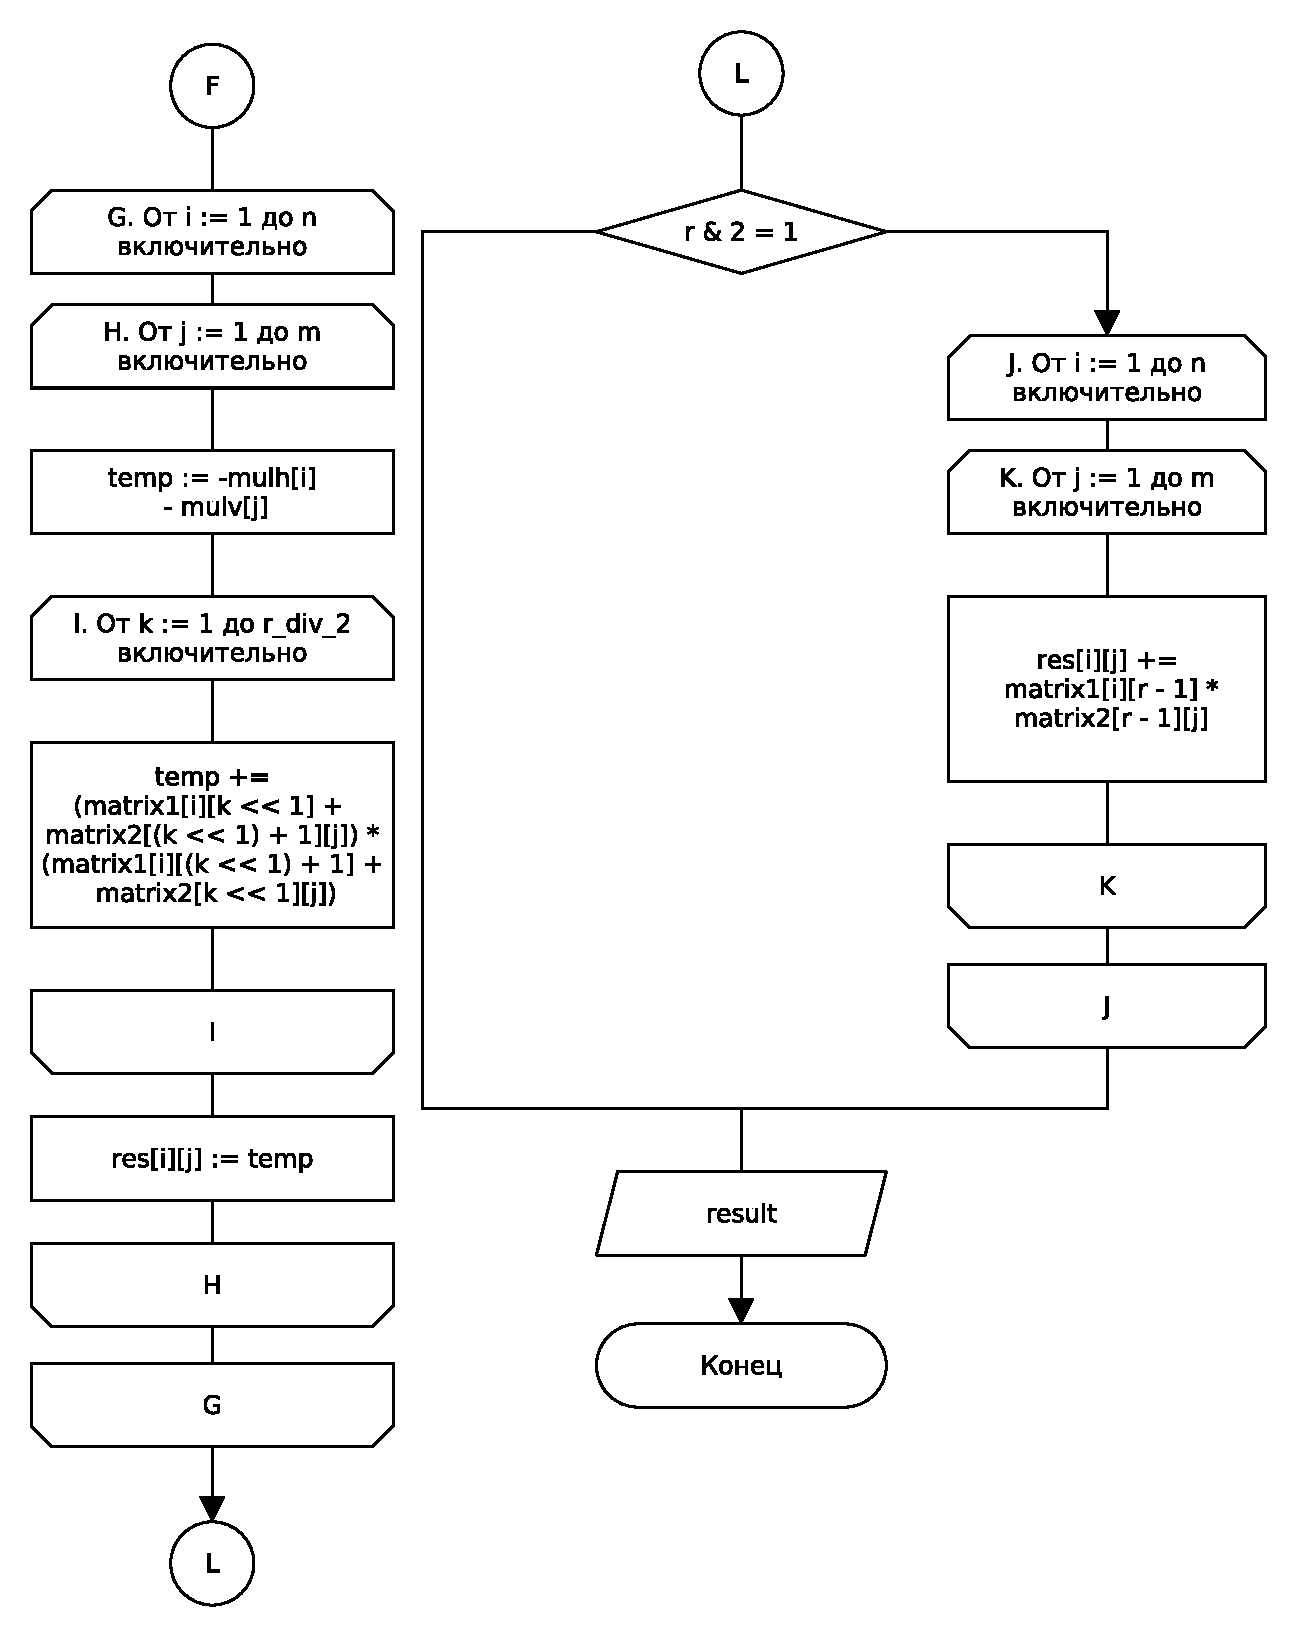
\includegraphics[scale=0.75]{pdf/owinograd-part2.pdf}
    \caption{Модифицированный алгоритм Винограда, часть 2}
\end{figure}

Имея схему модифицированного алгоритма Винограда, можем произвести оценку его сложности. Вначале схемы присутствует вычисление $r/2$ и присваивание полученного значения в переменную. Так как деление на 2 осуществляется при помощи двоичного сдвига, то итоговая стоимость данного выражения составляет 2.

Далее следуют два уже рассмотренных однотипных цикла с новой операцией присваивания и буферизацией вычисляемого значения вектора. С учётом произведённых изменений имеем общую стоимость первого цикла:
\begin{equation}
    1 + n \cdot{} (3 + 1 + 3 + \frac{r}{2} \cdot{} (2 + 15)) = 8.5nr + 7n + 1
\end{equation}

и второго:
\begin{equation}
    1 + m \cdot{} (3 + 1 + 3 + \frac{r}{2} \cdot{} (2 + 15)) = 8.5mr + 7m + 1
\end{equation}

Теперь рассмотрим стоимость модифицированного тройного цикла:
\begin{equation}
    \begin{gathered}
        1 + n \cdot{} (3 + m \cdot{} (4 + \frac{r}{2} \cdot{} (2 + 25) + 5) = 13.5nmr + 9nm + 3n + 1
    \end{gathered}
\end{equation}

Остается вычислить стоимость завершающего алгоритм ветвления. Цена условия равна 2. а стоимость блока, выполняемого в случае истинности этого условия, составляет:
\begin{equation}
    \begin{gathered}
        1 + n \cdot{} (3 + m \cdot{} (2 + 17)) = 19nm + 5n + 1
    \end{gathered}
\end{equation}

Таким образом имеем суммарную цену:
\begin{equation}
    13.5nmr + 9nm + 8.5nr + 8.5mr + 10n + 7m + 7 + Z
\end{equation}
где
\begin{equation}
Z = \left\{ \begin{array}{ll}
 19nm + 5n + 1, & \textrm{если r нечётно}\\
 0, & \textrm{иначе}\\
\end{array} \right.
\end{equation}

\section{Вывод}
По итогу проведённой оценки трудоёмкости разработанных алгоритмов можно сделать вывод, что при $n \to{} \infty{}$ алгоритм Винограда будет работать быстрее, чем стандартный алгоритм умножения матриц. В свою очередь модифицированный алгоритм Винограда теоретически должен работать быстрее алгоритма Винограда.

